% https://adrianb.io/2016/10/01/raymarching.html#introduction-to-raymarching
\chapter{Marcher}
% https://books.google.es/books?id=MNqRDwAAQBAJ&pg=PA13&dq=sphere+ray+marcher+graphics&hl=es&sa=X&ved=0ahUKEwj1sqWTgZvrAhUCxhoKHRwBCVIQ6AEIJzAA#v=onepage&q=sphere%20ray%20marcher%20graphics&f=false
Gracias a los avances tecnológicos y al incremento de la potencia de los micro-procesadores, a esto, unido la paralelización de tareas y dispositivos hardwares especializados como la \textit{GPU}, ha permitido que se pueda proponer esta técnica. Cada píxel de nuestra pantalla es calculado por una \textit{hebra} de la GPU, una especie de micro-procesador que trabaja de manera individual, sin memoria y sin intercomunicación con las demás. Todas ejecutan el mismo código, contiene información de la pantalla como la coordenada del pixel que está calculado, la resolución, etc. y devuelve un valor \textit{rgba}, en formato \textit{vec4}.\\\\
Existen técnicas para proyectar una escena en nuestras pantallas. Dentro de esta categoría de técnicas, encontramos las técnicas basadas en "rayos" (\textit{rays}). Para cada pixel de nuestra pantalla, "lanzaremos un rayo" desde un ojo, que es el nombre que recibe el origen de la cámara, en dirección al píxel, suponiendo que nuestra pantalla está en la escena. Si este rayo intersecta sobre una superficie, entonces podemos dibujarlo.\\\\
\begin{figure}[H]
  \centering
  \captionsetup{justification=centering}
  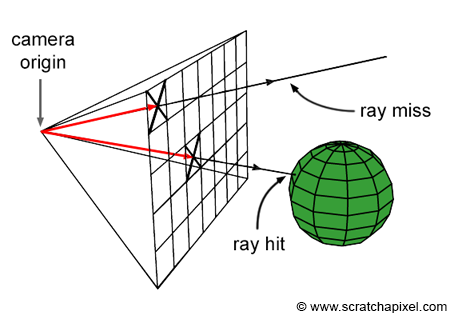
\includegraphics[width=0.6\textwidth]{secciones/imagenes/gpu.png}\label{fig:marcher}
  \caption{Pararelismo de la GPU en dibujado mediante rayos.}
\end{figure}
Definimos lanzar un rayo como aproximar con un vector o utilizar una recta para trazar una escena que encontramos desde el \textit{ojo} en dirección al píxel. Si utilizamos una recta, tratamos de la técnica \textit{raytracing}, que calcula de forma exacta la intersección con los objetos de la escena. Mientras si utilzamos un vector, trataremos de \text{raymarching}, que \textbf{aproxima} la intersección con la escena utilizando una modulación incremental del vector director.\\\\
Computacionalmente, aproximar, suele ser menos costoso que calcular de forma exacta el resultado. Por ello, vamos a utilizar la técnica de \textit{Raymarching}, para aproximar la escena y las \textit{funciones de distancia con signo} para crearla, esta técnica recibe el nombre de \textit{Spheremarching}, que se le ha atribuido el reconocimiento a John Hart en 1996 aunque  se cree que ya otros autores habían investigado acerca de la técnica presentada. \\\\
Utilizaremos el vector director del \textit{ojo} hacia el píxel, incrementando el módulo según el valor de distancia desde la cabeza del vector, de manera recursiva con un número de iteraciones máximas. Recibe el prefijo \enquote{\textit{Sphere}\textendash} ya que, por definición, podemos generar una esfera de radio \(r\), sobre la cabeza del vector, con valor de la función de distancia \(r=sdf(x,y,z)\). Tal que, la esfera, no contine ningún punto en su interior.\\\\
Para fijar el número de iteraciones, se recomienda utilizar una potencia de \(2\). Cuanto mayor sea este número, mejor será la aproximación, aunque, mayor el gasto computacional. No existe un valor por defecto, este dependerá de la escena utilizada y será elegido de forma empírica.\\
Vamos a definir las \textbf{condiciones de parada} de este algoritmo.
\begin{enumerate}
    \item Estar cerca de la isosuperficie. Como el radio de la esfera, indica la distancia a la isosuperfice más cercana, utilizaremos un umbral \(\epsilon\), muy pequeño, para definir la distancia a la que consideramos isosuperficie, en un modelo exacto, \(\epsilon=0.0\).
    \item Superar una cierta distancia recorrida, esta distancia actuará como plano trasero, en caso de superarlo, devolveremos la distancia impuesta para dicho plano. 
    \item Superar el número de iteraciones máximas, en caso afirmativo, devolveremos la distancia al plano trasero.
\end{enumerate}
 En los casos en los que se devuelve la distancia al panel trasero, recibirán el nombre de "\textit{fallo}", que representa un pixel que no ha podido trazar una isosuperficie. Pudiéndose considerar, el fondo de la escena, existen algunos casos, en los que encerraremos nuestra escena en una isosuperficie que actuará como fondo.
\begin{figure}[H]
  \centering
  \captionsetup{justification=centering}%,margin=2cm
  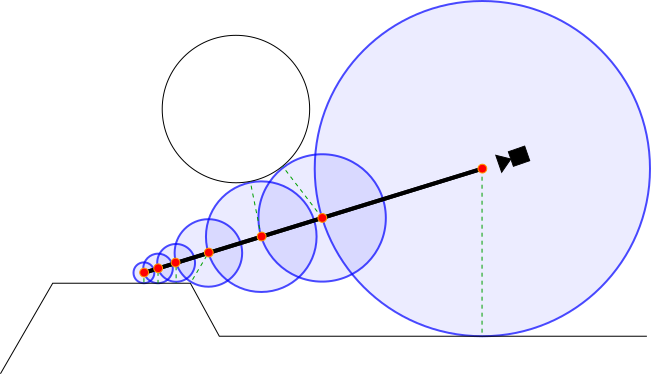
\includegraphics[width=0.8\textwidth]{secciones/imagenes/raymarching.png}\label{fig:spheremarcher}
  \caption{Ejemplo del algoritmo \textit{Spheremarching}}
\end{figure}
\newpage
\begin{lstlisting}
#define PASOS 128 // Número Máximo de Iteraciones.
#define EPSILON 0.001
#define MAXIMO 20.0 // Distancia del Plano Trasero.

// Pasamos el origen del ojo y la dirección, nos devuelve la distancia al objeto más cercano del ojo en dicha dirección.
float SphereMarching(
    vec3 ojo, 
    vec3 direccion
){
    float distancia = 0.0;
    // Realizamos "PASOS" iteraciones de marching.
    for(int i = 0; i < PASOS; ++i){
        // Calculamos el vector (rayo).
        vec3 rayo = ojo + direccion * distancia;
        // Aproximamos el radio de la esfera más próxima a una isosuperficie
        float radio = escena_sdf(rayo);
        // Si el radio (distancia mínima a la isosuperficie), es muy pequeña, podemos decir que estamos sobre la distancia y devolvemos el módulo del rayo.
        if(radio < EPSILON){
            return distancia;
        }
        // Incrementamos la distancia recorrida si no estamos cerca de la isosuperficie.
        distancia += radio;
        // Comprobamos que no se haya superado la distancia de dibujado máximo. Podemos considerarlos el fondo de la escena.
        if(distancia >= MAXIMO) break;
        return MAXIMO;
    }
}
\end{lstlisting}
\newpage
Como ya se ha comentado antes, este algoritmo es aplicado para cada pixel de la pantalla, si el valor devuelto por el \textit{Marcher} es distinto a un \textit{fallo}, sabremos que estamos muy próximos a una isosuperficie y así, dibujarlo. En caso contrario, lo consideraremos fondo. Con la distancia devuelta, podemos posicionarlo en nuestra escena ya que el valor devuelto es la distancia aproximada a la isosuperficie, por lo que, el vector a dicho punto, aproximado, será:
\[ \Vec{p} = \Vec{ojo} + distancia \cdot  \Vec{direccion} \]
Como ya hemos comentado, \textit{Shadertoy} nos ofrece un entorno para trabajar, además de un pequeño código de ejemplo, el cual modificaremos para adaptarlo al \textit{Marcher}.
\begin{lstlisting}
void mainImage( out vec4 fragColor, in vec2 fragCoord )
{
    // Normalized pixel coordinates (from 0 to 1)
    vec2 uv = fragCoord/iResolution.xy;

    // Time varying pixel color
    vec3 col = 0.5 + 0.5*cos(iTime+uv.xyx+vec3(0,2,4));

    // Output to screen
    fragColor = vec4(col,1.0);
}
\end{lstlisting}
Podemos observar tres variables importantes, que se han comentado anteriormente.
\begin{enumerate}
    \item \textit{fragColor}. Se trata de una variable de \textbf{salida}, es el valor del pixel, es decir, una 4-upla \textit{rgba} de tipo \textit{vec4}. Cada elemento está en el intervalo \([0,1]\).
    \item \textit{fragCoord}. Es una variable de \textbf{entrada}, la coordenada del pixel en pantalla, donde la primera componente representa la coordenada \(x\) y la segunda, la \(y\).
    \item \textit{iResolution}. Contiene el ancho y el alto de la pantalla.
\end{enumerate}
La pantalla en realidad nos referimos al donde se dibuja el resultado.
\newpage
\begin{lstlisting}
void mainImage(
    out vec4 fragColor, 
    in vec2 fragCoord
){
    // Normalizamos las coordendas y las reescalamos para mantener el ratio de aspecto. Transladamos al centro de la pantalla.
    vec2 uv = (fragCoord - iResolution.xy * 0.5) / min(iResolution.y, iResolution.x);
    // Definimos el ojo y la pantalla, que se encuentra en nuestra escena.
    vec3 ojo = vec3(0.0, 0.0, -1.0);
    vec3 pantalla = vec3(uv, 0.0);
    // La dirección del rayo es el vector normalizado que apunta desde el ojo hasta la pantalla (píxel).
    vec3 direccion = normalize(pantalla-ojo);
    // Con esto, ya podemos utilizar nuestro Sphere marcher.
    float distancia = SphereMarching(ojo, direccion);
    // El marcher nos ha devuelto una distancia inferior al plano trasero, estamos sobre la isosuperficie.
    if(distancia < MAXIMO){
        // Estamos aproximadamente sobre la isosuperficie.
        // La posición aproximada es la siguiente.
        vec3 p = ojo + direccion * distancia;
        // Utilizamos el color blanco para dibujar la isosuperficie.
        fragColor = vec4(1.0);
    }else{ // El marcher ha fallado.
        // El color negro para pintar el fondo.
        fragColor = vec4(vec3(0.0), 1.0);
    }
}
\end{lstlisting}
\newpage
Si intentáramos ejecutar este código, veríamos que no compilaría, esto es debido a que no hemos definido aún nuestra escena. La función \textit{escena\_sdf} que se encuentra dentro de la función \textit{SphereMarching}, contiene nuestra escena como una \textit{Funcíon de distancia con Signo}, vamos a definir la escena más simple, aunque en capítulos posteriores, veremos formas de crear nuestras propias escenas y funciones de distancia con signo.
\begin{lstlisting}
/* 
No vamos a entrar, aún, en como se define una escena mediante Funciones de Distancia con Signo.
Aunque el siguiente código, representa:
Una esfera en el la coordenada (0,0,0) de radio 0.2 unidades.
*/
float escena_sdf(vec3 p){
    return length(p - vec3(0.0)) - 0.2;
}
\end{lstlisting}
Veamos una pequeña pincelada de como se ha definido esta función. Se calcula el módulo del punto \(\Vec{p}\), esto define una \textit{Función de Distancia con Signo} positiva y cuya isosuperficie es únicamente un punto, \(S=\{(0,0,0)\}\).\\Es fácil observar que si restamos \(r\) al la distancia, estamos creando una isosuperficie esférica de radio \(r\). Aquellos puntos cuya distancias valen \(r\), acabarán anulándose y definiendo la \textit{isosuperficie}. Las distancias inferiores, tomarán valores negativos y los superiores, positivos.
\[S=\{\Vec{q} \in \mathbb{R}^3 / SDFEsfera_r(\Vec{q})=0\}\]
\[ SDFEsfera_r(\Vec{p})=\vert\vert\Vec{p}\vert\vert - r  \]
\begin{figure}[H]
  \centering
  \captionsetup{justification=centering}%,margin=2cm
  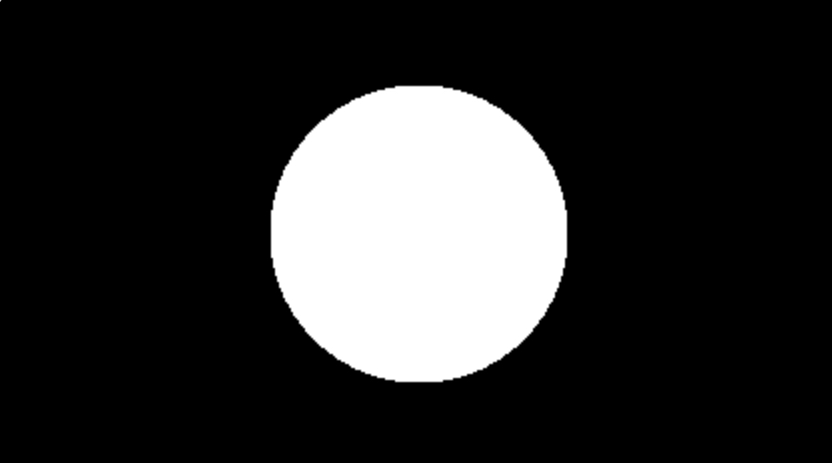
\includegraphics[width=0.8\textwidth]{secciones/imagenes/sdf1.jpeg}\label{fig:hello}
  \caption{"Hola mundo" del algoritmo \textit{SDF}.}
\end{figure}
Al solo utilizar dos colores, blanco y negro, no tenemos sensación de profundidad, esto se conseguirá utilizando un modelo de iluminación, que incluyen luces y sombras.